\documentclass[a4paper,14pt]{extreport}
\usepackage[utf8]{inputenc}
\usepackage[T1]{fontenc}
\usepackage{scrextend}
\usepackage{amsmath}
\usepackage{amssymb}
\usepackage{makeidx}
\usepackage{graphicx}
\usepackage[russian]{babel}
\usepackage{indentfirst}
\usepackage{caption2}
\usepackage{listings}
\usepackage{color}   %May be necessary if you want to color links
\usepackage{hyperref}
\hypersetup{
	colorlinks=false, %set true if you want colored links
	linktoc=all,     %set to all if you want both sections and subsections linked
	linkcolor=blue,  %choose some color if you want links to stand out
}

\usepackage[left=2.50cm, right=2.00cm, top=2.00cm, bottom=2.00cm]{geometry}
\linespread{1.5}

\lstdefinestyle{bash}{basicstyle=\ttfamily\footnotesize,
	frame=tb, 
	aboveskip=5mm,
	belowskip=2mm,
	breaklines=true,
	breakatwhitespace=true,
	tabsize=3}

\lstdefinestyle{stdout}{basicstyle=\ttfamily\footnotesize,
	frame=single, 
	aboveskip=5mm,
	belowskip=2mm,
	breaklines=true,
	breakatwhitespace=true,
	tabsize=3}


\author{Павел Горбоконенко}
\graphicspath{ {./images/} }
\setcounter{tocdepth}{0}

\newcommand{\ssubsection}[1]{%
	\subsection[#1]{\normalsize\normalfont#1}}

\begin{document}
	\renewcommand{\figurename}{Рисунок}
	\renewcommand{\captionlabeldelim}{.}
	\renewcommand{\chaptername}{Лабораторная работа №}
	\makeatletter
	\renewcommand\subsection{\@startsection{subsection}{2}{\z@}
		{-3.25ex\@plus -1ex \@minus -.2ex}%
		{-1.5ex \@plus .2ex}%
		{\normalfont\normalsize\bfseries}}
	\renewcommand\subsubsection{\@startsection{subsubsection}{3}{\z@}
		{-3.25ex\@plus -1ex \@minus -.2ex}%
		{-1.5ex \@plus .2ex}%
		{\normalfont\normalsize\bfseries}}
	\makeatother
	
	\rmfamily
	\begin{titlepage}
	\begin{center}		
		\textbf{РТУ МИРЭА (ТУ)} \\
		Центр проектирования интегральных схем, устройств наноэлектроники и микросистем 
		
		\vspace{5.5cm}
		
		\Large
		\textbf{Методическое пособие по лабораторным работам}
		
		\vspace{0.5cm}
		
		«Багет-ПЛК1-01» \\
		(ОС Linux, Debian 10) \\
				
		\vfill
				
		\vspace{0.8cm}
		
		
\includegraphics[width=0.4\textwidth]{mirea}
		
		\Large
		Москва\\
		2023
		
	\end{center}
\end{titlepage}	

	\tableofcontents	

	\addcontentsline{toc}{chapter}{Введение}
\chapter*{Введение}
Методическое пособие описывает основные шаги по разработке программного обеспечения для встраиваемых систем. В качестве целевой платформы используется плата «Багет ПЛК1-01» с установленным микроконтроллером Комдив-МК К5500ВК018, производства ФГУ ФНЦ НИИСИ РАН. В состав К5500ВК018 входит суперскалярное 64-разрядное RISC микропроцессорное ядро с архитектурой КОМДИВ64 (MIPS64-совместимая), включая сопроцессор вещественной арифметики (IEEE754), кэш-память первого уровня (16+16 кБ), кэш-память второго уровня (128 кБ), буфер трансляции виртуальных адресов на 64 адреса, контроллер динамической памяти DDR3L, восемь таймеров-счетчиков, сторожевой таймер, часы реального времени, два контроллера Ethernet 10/100, контроллеры последовательных интерфейсов RS-232C (4 шт.), I2C (2 шт.), SPI (3 шт.), QSPI, CAN 2.0 (2 шт.), USB 2.0. Серийный выпуск начат в 2021 году. 

ПЛК1-01 выполнен в виде печатной платы без корпуса, на которой расположены
соединители для подключения первичного электропитания и внешних устройств, органы
управления (пользовательские кнопки SW1, SW2), светодиодные индикаторы (VD1 –
VD5), перемычки для управления режимами работы ПЛК1-01 (SA4, SA5, SA6, SA7, SA9). 

\begin{center}
	\begin{tabular}{||c | c||}
		\hline
		Назначение & Вывод процессора \\ [0.5ex]
		\hline\hline
		Кнопка SW2 & GPIOD 6 \\
		\hline
		Зелёный светодиод VD2 & GPIOD 4 \\
		\hline
		Жёлтый светодиод VD5 & GPIOD 5 \\
		\hline
	\end{tabular}
\end{center}

Для организации питания часов реального времени (RTC) микроконтроллера
К5500ВК018 при отсутствии основного питания предусмотрена установка
автономного элемента питания – батарейки типа CR2032 +3 В.
Расположение соединителей, органов управления и индикаторов ПЛК1-01
приведено на рисунке \ref{fig:fig1}, назначение выводов на некоторых из разъёмов приведены на рисунке \ref{fig:fig2}.

\begin{center}
	\begin{figure}
		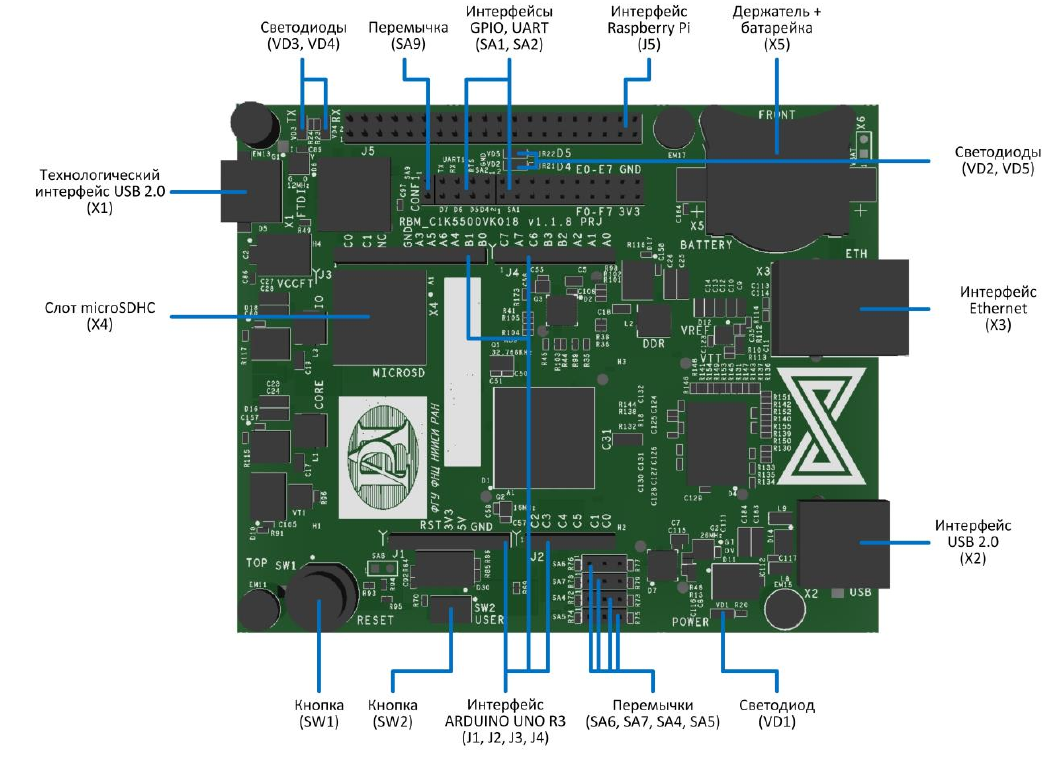
\includegraphics[width=\textwidth]{pic_01}
		\caption{Расположение портов ввода-вывода}
		\label{fig:fig1}
	\end{figure}
\end{center}

\begin{center}
	\begin{figure}
		\centering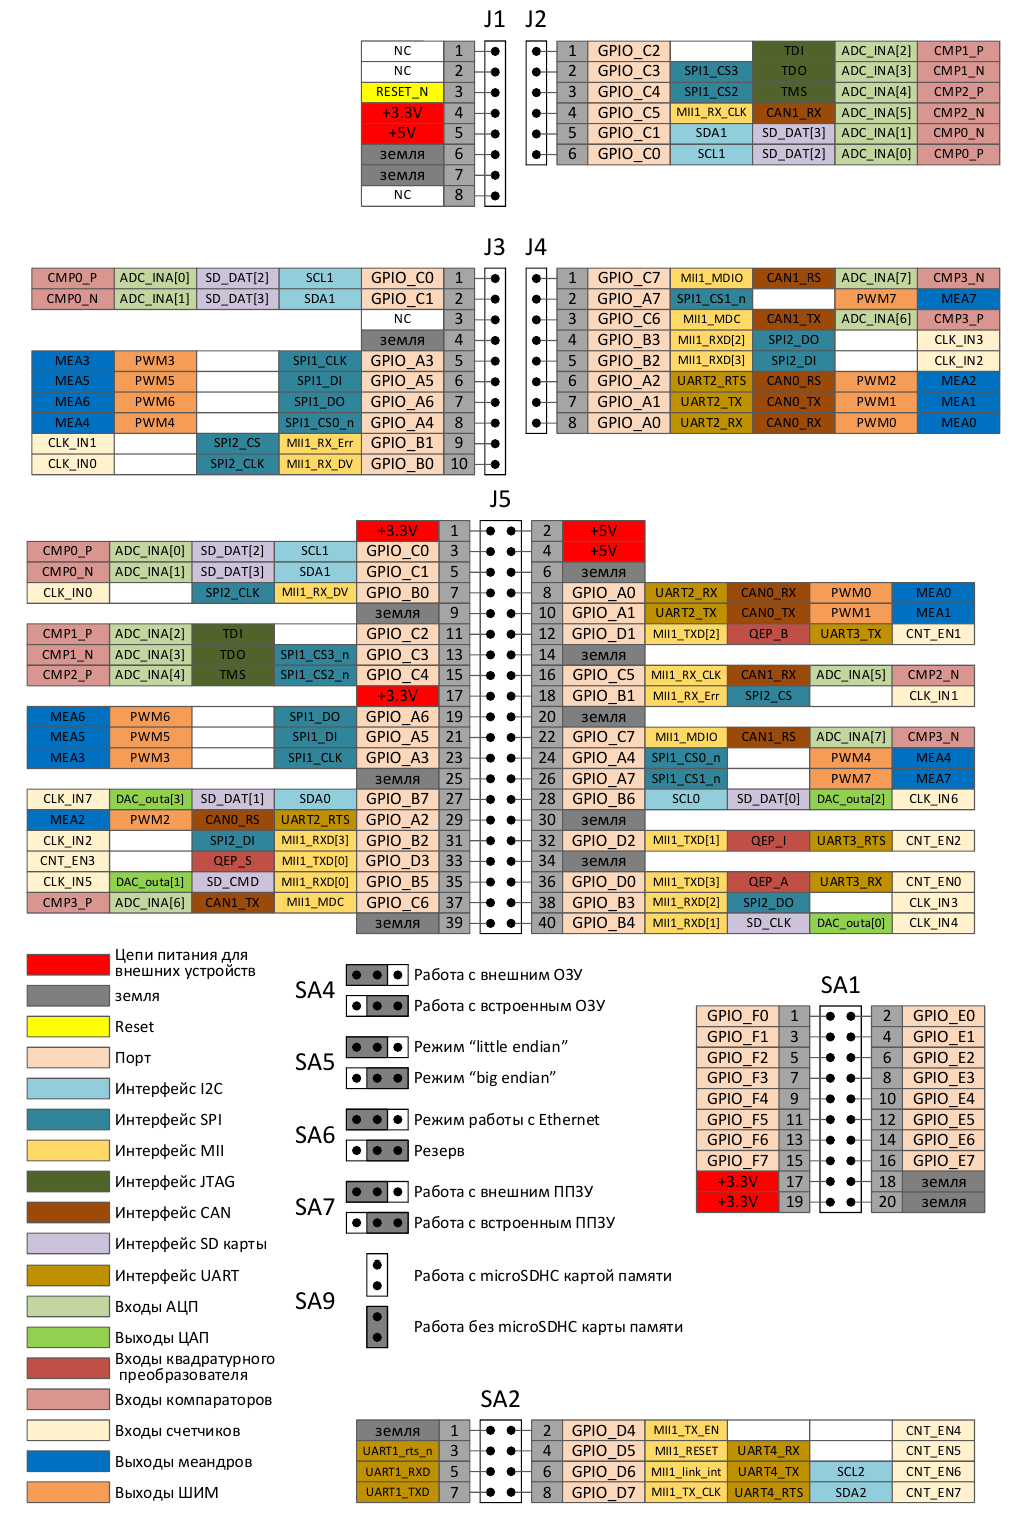
\includegraphics[width=\textwidth]{pic_02}
		\caption{Разводка выводов процессора по разъёмам ввода-вывода}
		\label{fig:fig2}
	\end{figure}
\end{center}

\vspace{10mm}
\section*{Переходная плата}
Для удобства подключения к интерфейсам целевой платы, была разработана переходная плата, с выведенными сигнальными линиями, сгруппированными по интерфейсам (рисунок \ref{fig:fig3}).  

\begin{figure}[hbt!]
	\centering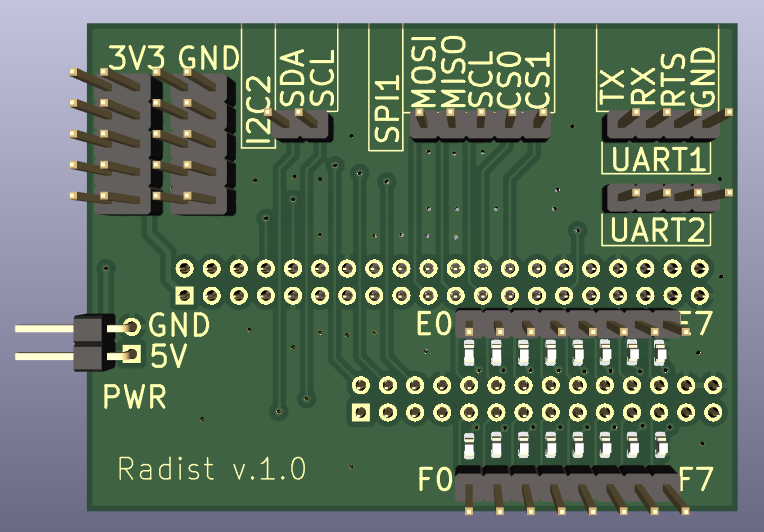
\includegraphics[width=\textwidth]{pic_03}
	\caption{Переходная плата}
	\label{fig:fig3}
\end{figure}

UART2 можно использовать как для работы с интерфейсом UART2, так и для работы с интерфейсом CAN0. Выводы GPIO банков E и F дублируются на светодиоды для отладочных целей. При необходимости, можно подключать к выводам кнопки, или использовать их для формирования управляющих сигналов для модулей. Также обратите внимание, что одна из сигнальных линий I2C интерфейса используется кнопкой SW2 на плате, по этой причине не стоит использовать кнопку при активации этого нтерфейса.    


\section*{Как запускается Linux?}
Для запуска ОС Linux в общем случае должны пройти следующие этапы:
\begin{enumerate}
	\item  ROM BOOT — запуск встроенного загрузчика, определяющего источник дальнейшей загрузки. Этот код нельзя исправить его работа и формат образа (заголовки, значение бит и прочее) зависит от производителя.
	
	\item First Stage Bootloader (FSBL) — загрузчик первой ступени, задача этого загрузчика, начальная инициализация процессора, и загрузка пользовательского кода в DDR память. Данный загрузчик опциональный, и у некоторых производителей может отсутствовать. Работает из встроенной RAM памяти процессора.
	
	\item Second Stage Bootloader (SSBL) — это загрузчик второго уровня, задача которого заключается в подготовке системы к запуску ядра Linux, с пользовательскими параметрами (точка монтирования rootfs, скорость работы терминала для логов и прочее). Наиболее распространённый вариант загрузчика проекта Das U-Boot. В целевой плате используется другой загрузчик, набирающий популярность — Barebox.
	
	\item Kernel — на этом этапе за работу процессора отвечает ядро, происходит финальная конфигурация, активация дополнительный ядер (если они есть и активирована функция многоядерной поддержки), монтирование rootfs, запуск сервисов и прочее.
\end{enumerate}


\section*{Описание окружения}
Для работы с платой используется виртуальная машина на базе Kubuntu 20.04. На виртуальной машине установлены пакеты для компиляции кода под Linux для MIPS64 архитектуры mips64el-linux-gnu-gcc (C компилятор) и mips64el-linux-gnu-g++ (C++ компилятор), компилятор дерева устройств device-tree-compiler, архив с заголовочными файлами ядра Linux установленного на плате, утилита debootstrap, IDE VSCode и прочие полезные инструменты. 

Имя пользователя \textbf{student} пароль \textbf{usrstudent}. Пользователь поддерживает работу через sudo (получение прав суперпользователя он же администратор).

В конце некоторых работ есть задания для самостоятельного выполнения. При этом есть простые задачи, предполагающие незначительное изменение кода, а также есть помеченные *. Последние выполняются по желанию, при этом нужно быть готовым, что придётся активно пользоваться поиском, и расходовать клетки серого вещества.

\textbf{ВНИМАНИЕ!} Запомните, что далее по тексту, если просят выполнить команду, в начале которой написано \textbf{\$} , значит команду нужно выполнить на целевой плате, а если с \textbf{\#} - в консоли виртуальной машины. При этом \$ или \# писать не нужно! 

Если команда заканчивается символом \verb!\! и на следующей строчке есть запись, то это запись относиться к одной команде, Вы можете записать как видите, так как символ \verb!\! в консоли Linux означает многострочную команду или, опустив символ \verb!\!, продолжить вводить текст приведённый на следующей строке методички.\\


\textbf{Примеры:}

Авторы хотят, что бы Вы в консоли виртуальной машины (ВМ) записали echo Hello и нажали кнопку Enter:

\begin{lstlisting}[style=bash]
# echo Hello 
\end{lstlisting}

Авторы хотят, что бы Вы в консоли целевой платы записали echo FOOBAR и нажали кнопку Enter:

\begin{lstlisting}[style=bash]
$ echo FOOBAR
\end{lstlisting}

Авторы хотят, что бы Вы в консоли виртуальной машины (ВМ) написали очень длинную команду (да-да, вечер не обещает быть томным) и нажали кнопку  Enter:

\begin{lstlisting}[style=bash]
# echo \
FOOBAR 
\end{lstlisting}
	\chapter{Установка ОС на целевую платформу}
\textbf{Цель:} Установить дистрибутив Debian 10 на целевую платформу.

\textbf{Описание:} Нужно понимать, что ОС Linux делиться на две части. Ядро (Kernel) и файловую систему (rootfs). Ядро определяет какие возможности по взаимодействию с железом доступны пользователю и приложениям. Rootfs определяет какие инструменты есть в системе, порядок инициализации, запуска сервисов и прочие прикладные штуки. Дистрибутив это в большей степени наполнение rootfs. Не каждый дистрибутив имеет поддержку иной от x86 архитектур.

Для установки debian воспользуемся инструментом под названием debootstrap, который отвечает за создание rootfs. Подробнее про этот инструмент, и возможности по его управлению, Вы можете найти на wiki проекта Debian.
\section{Подготовка rootfs}

\subsection{}Запустите виртуальную машину. Логин и пароль для входа: student / usrstudent.

\subsection{} Запустите консоль нажав комбинацию клавиш на клавиатуре \textbf{Ctrl+Alt+T} \\

\textbf{Внимание!} В консоли есть возможность автоматического продолжения ввода. Для этого необходимо ввести первые символы команды, или пути, и нажать клавишу TAB. Ввод продолжиться до тех пор, пока не появиться неопределённостью (к примеру у Вас есть два файла foo\_bar1 и foo\_bar2, при нажатии TAB будет вставлен текст до цифры). Двойное нажатие TAB приведёт к выводу всех возможных вариантов продолжения, если таковые есть.

\subsection{}Создайте и перейдти в рабочий каталог в котором будет создан образ rootfs.
\begin{lstlisting}
# mkdir -p $BAGET/lab_01
# cd $BAGET/lab_01 
\end{lstlisting}

\subsection{} Запустите утилиту debootstrap (при необходимсоти введите пароль usrstudent):
\begin{lstlisting}
# sudo debootstrap --include=aptitude,nano,wget \
--foreign \
--arch=mips64el buster rootfs
\end{lstlisting}
\textit{-{}-include=A,B,C..} - добавить в сборку указанные пакеты \\
\textit{-{}-foreign} — только сгенерировать наполнение, применяется когда архитектура на которой запускается утилита отлична от архитектуры назначения. \\
\textit{-{}-arch=mips64el} — указываем целевую архитектуру \\
\textit{buster} — версия сборки \\
\textit{rootfs} — путь к папке назначения, где будут размещены файлы \\

\subsection{} Для продолжения установки, нам понадобиться утилита qemu позволяющая эмулировать различные архитектуры. Скопируем исполняемый файл qemu:
\begin{lstlisting}
# sudo cp /usr/bin/qemu-mips64el-static ./rootfs/usr/bin
\end{lstlisting}
и перейдём в созданную rootfs (привет дедушка контейнеров, chroot)
\begin{lstlisting}
# sudo chroot ./rootfs
\end{lstlisting}

\section{Настройка rootfs}

\subsection{} Завершим работу debootstrap
\begin{lstlisting}
# export LANG=en_US.UTF-8
# /debootstrap/debootstrap --second-stage
\end{lstlisting}

\subsection{}Добавим источники для установки ПО, для этого выполним следующие команды 
\begin{lstlisting}
# echo deb http://ftp.debian.org/debian buster \
main contrib non-free  >> /etc/apt/sources.list

# echo deb-src http://ftp.debian.org/debian buster \
main contrib non-free >> /etc/apt/sources.list

# echo deb http://ftp.debian.org/debian buster-updates \
main contrib non-free >> /etc/apt/sources.list

# echo deb-src http://ftp.debian.org/debian buster-updates \
main contrib non-free >> /etc/apt/sources.list
\end{lstlisting}

\subsection{} Обновим список, и установим ряд приложений
\begin{lstlisting}
# apt-get update
# apt-get install -y dialog sudo less i2c-tools evtest mc \
openssh-server resolvconf hwinfo net-tools
\end{lstlisting}

\subsection{}Зададим пароль для root пользователя
\begin{lstlisting}
# passwd root
\end{lstlisting}
После чего введите root (внимание, курсор двигаться не будет, это политика безопасности Linux, при вводе пароля курсор не перемещается, что бы нельзя было установить количество символов). И нажмите Enter

Затем Вас попросят повторить пароль, снова введите root и нажмите Enter
	\chapter{Ознакомительная}
\textbf{Цель:} Запустить плату, подключиться к ней через консоль и по сетевому интерфейсу, работа с кнопкой и светодиодами через sysfs.

\vspace{5mm}
\textbf{Описание:} работа с ОС Linux на целевой платформе мало чем отличается от работы с данной ОС на обычном компьютере. Среди особенностей можно выделить наличие меньшего набора инструментов, и рабочих программ, что делается для экономии свободного места, и ускорения загрузки ОС. Так же может отсутствовать привычный рабочий стол, а вся работа сводиться к взаимодействию через рабочий терминал, она же консоль. Для подключения к консоли можно воспользоватся интерфейсом UART (он же COM порт, или последовательный порт), или при помощи сетевого соединения (ssh или реже telnet). 

При этом нужно понимать, что возможность работы через консоль настраивается, и не всегда может быть доступна по-умолчанию (обычно возможность сетевого подключения отключают, для повышения безопасности). 

\section{Запуск и подключение к устройству}

\subsection{}Запустите виртуальную машину. Логин и пароль для входа: student / usrstudent.

\subsection{}Подключите по USB плату к ПК. Проверьте, и при необходимости подключите USB устройство FTDI RBM\_C1K5500VK018 к виртуальной машине (меню Device→USB).

\subsection{}Откройте программу gtkterm, и подключитесь к порту /dev/ttyUSB1, или откройте консоль в виртуальной машине, и вызовете утилиту minicom.

\subsection{}Если в окне терминала нет текста, нажмите клавишу Enter на клавиатуре. Вы должны увидеть следующий вывод:
\begin{center}
	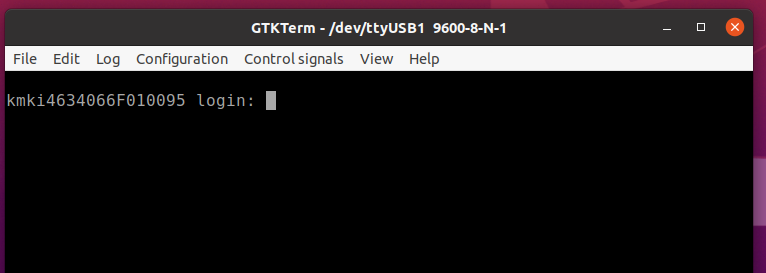
\includegraphics[width=\textwidth]{pic_08}
\end{center}
Вы подключились к консоли устройства. Введите логин root и пароль root.

\section{Подключение по сетевому интерфейсу}

Рассмотрим какие шаги необходимо выполнить, для того, что бы можно было организовать сетевое подключение к плате, для получение доступа к консоли и файловой системе через SSH соединение. Так же настройки, которые будут выполнены в данном разделе помогут в дальнейшем копировать файлы на плату через команду scp.

\subsection{}Проверьте текущие настройки интерфейса eth0 выполнив команду: 
\begin{lstlisting}[style=bash]
$ ip addr show dev eth0 
\end{lstlisting}
убедитесь, что в выдаче появилась строчка: 
\begin{lstlisting}[style=stdout]
	...
inet 192.168.100.200/24 scope global eth0 
	...
\end{lstlisting}
Если inet адрес отличается, то удалите текущий адрес (вместо <inet\_val> впишите адрес, который отобразился в консоли)
\begin{lstlisting}[style=bash]
$ ip addr del <inet_val> dev eth0
\end{lstlisting}
затем установите новый адрес командой 
\begin{lstlisting}[style=bash]
$ ip addr add 192.168.100.200/24 dev eth0
\end{lstlisting} 
Для активации изменения необходимо переподключится, для чего выполните следующие команды
\begin{lstlisting}[style=bash]
$ ip link set eth0 down
$ ip link set eth0 up
\end{lstlisting} 

\subsection{}Проверьте, что на плате запущен SSH сервер. Проверить открытые порты устройства, выполнив команду: 

\begin{lstlisting}[style=bash]
$ netstat -tulpn | grep LISTEN
\end{lstlisting} 
\begin{center}
	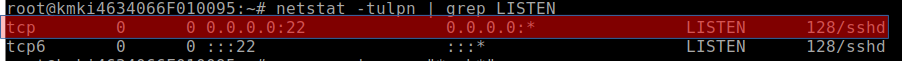
\includegraphics[width=\textwidth]{pic_09}
\end{center}
Если вывода, как на картинках выше не появилось, то выполните команду: 
\begin{lstlisting}[style=bash]
$ systemctl start sshd 
\end{lstlisting}
и проверьте снова. 

\subsection{}\label{lab2:ref1}Заходить через сеть в пользователя root не безопасно, поэтому создадим пользователя для дальнейшей работы через сетевой интерфейс, для этого введите следующие команды (пароль для пользователя netuser - usrnetuser):
\begin{lstlisting}[style=bash]
$ useradd -s /bin/bash -m netuser
$ passwd netuser
\end{lstlisting}

Первая команда для создания нового пользователя netuser с созданием домашнего каталога (/home/netuser) и также назначаем для него интерпретатора команд bash. 

\subsection{}Подключите сетевой шнур к рабочему ПК и плате

\subsection{}Откройте на виртуальной машине консоль, нажав на клавиатуре комбинацию клавиш Ctrl+Alt+T. 

\subsection{}\label{lab2:ref2}В открывшемся окне терминала введите команду: 
\begin{lstlisting}[style=bash]
# ssh netuser@192.168.100.200
\end{lstlisting}

\subsection{}Будет предложено ввести пароль пользователя, вводим тот, что установили в пункте \ref{lab2:ref1} и получаем доступ к терминалу платы.

Если вместо ввода пароля, в консоли появилась надпись похожую на:
\begin{lstlisting}[style=stdout]
The authenticity of host '192.168.100.200 (192.168.100.200)' can't be established.
ECDSA key fingerprint is SHA256:+OSEJhr2dIiTvlWZxq5fZ0UFdYYY+egbTgabe6F7zZE.
Are you sure you want to continue connecting (yes/no/[fingerprint])?
\end{lstlisting}
Введите yes и нажмите Enter, и повторно ведите пароль.
\\\\
Если же получите вывод как на картинке ниже
\begin{center}
	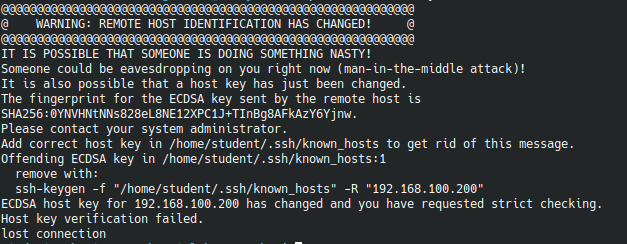
\includegraphics[width=\textwidth]{pic_10}
\end{center}
Выполните команду 
\begin{lstlisting}[style=bash]
$ ssh-keygen -f "/home/student/.ssh/known_hosts" -R "192.168.100.200"
\end{lstlisting}
и вернитесь к пункту \ref{lab2:ref2}

\subsection{}Завершите сеанс, введя команду exit 

\section{Аппаратный Hello world }

В этой части будет показано, как можно управлять выводами микроконтроллера, для переключения светодиодов и считывания состояния кнопки, при помощи виртуальной файловой системы sysfs.

Для работы с периферией в ОС Linux помимо прочего есть две виртуальные файловые системы: procfs (точка входа /proc) и sysfs (точка входа /sys).  

Sysfs экспортирует в пространство пользователя информацию ядра Linux о присутствующих в системе устройствах и драйверах, что позволяет не только считывать значение (например с датчиков температуры), но и менять поведение, если это было заложено разработчиками драйвера.

За формирование наполнения виртуальных файловых систем отвечают в том числе и модули ядра Linux, которые выполняют роль драйвера, если речь идёт про взаимодействие с периферийным модулями.

\subsection{}Перейдите в каталог /sys/class/gpio:
\begin{lstlisting}[style=bash]
$ cd /sys/class/gpio
\end{lstlisting}

\subsection{}Выведите список фалов и каталогов в текущей директории: 
\begin{lstlisting}[style=bash]
$ ls -l
\end{lstlisting}
\begin{center}
	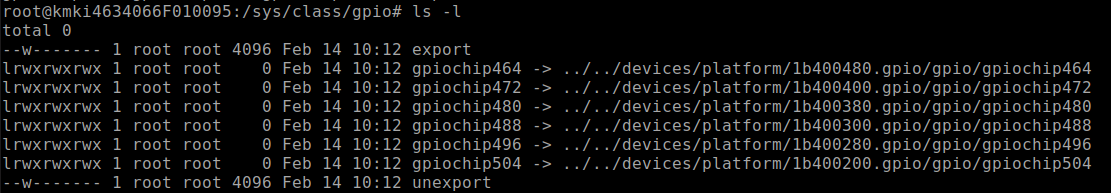
\includegraphics[width=\textwidth]{pic_11}
\end{center}

Первый и последний файлы используются для того, что бы подключать (export) драйвер для управления отдельным выводом в файловую систему sysfs или отключать (unexport). 

Далее идёт серия символьных ссылок на каталоги, каждый из которых описывает один банк сигналов ввода-вывода общего назначения (GPIO). Тут нужно отметить, что в рабочем чипе присутствует 6 банков (A, B, C, D, E и F), по 8 выводов в каждом, по этой причине мы видим 6 каталогов.  

Обратите внимание на имена каталогов, внутри каталога platform. Первая часть имени является базовым адресом периферийного модуля, отвечающего за управление банком выводов. Первому банку выводов A соответствует адрес 0x1B400200, остальные по возрастанию. 

Так же обратите своё внимание, что в данной сборке, номера файлов gpiochip уменьшаются(!), при продвижении от выводов в банке A к выводам в банке F.

\subsection{}У выводов общего назначения в рамках ядра Linux нумерация сквозная. Таким образом, можно определить, что вывод подключённый к кнопке SW2 (банк D, вывод 6) находиться под номерам 486 (480 + 6).  Выполним следующую команду:
\begin{lstlisting}[style=bash]
$ echo 486 > export
\end{lstlisting}

\subsection{}Выполните эту же команду для экспорта пары выводов банка F (504 и 505) 

\subsection{}После каждой команды будет создан каталог ./gpioXXX где вместо XXX будет номер вывода. Если зайти в любой из этих каталогов, то можно увидеть там одинаковый набор файлов, но нас интересуют следующие: 
\begin{itemize}
\item direction — задаёт направление вывода (in вывод настроен как вход, out — как выход)
\item value — если вывод настроен как вход, то читая этот файл можем узнать уровень логического сигнала на выводе. Если настроен на выход, то запись в этот файл 0 или 1 будет устанавливать соответствующий уровень выходного сигнала.
\end{itemize}

\subsection{}Так как два вывода банка F управляют светодиодами, изменим значение в файле direction  для них на out
\begin{lstlisting}[style=bash]
$ echo out > gpio504/direction
$ echo out > gpio505/direction
\end{lstlisting}

\subsection{}Переключать светодиоды можно записью 0 или 1 в файл value соответствующего вывода
\begin{lstlisting}[style=bash]
$ echo 1 > gpio504/value
$ echo 0 > gpio504/value
\end{lstlisting}

\subsection{}Для взаимодействия с кнопкой менять ничего не нужно. Для удобства отладки запустить считывание файла через утилиту watch позволяющую выполнять заданную команду через указанный интервал времени.

\begin{lstlisting}[style=bash]
$ watch -n 1 cat gpio486/value
\end{lstlisting}

После чего можете нажимать кнопку, и смотреть как меняется значение считанное из файла. В данном примере файл будет считываться каждую секунду (из-за параметра -n 1 переданного при запуске утилите watch).  

\subsection{}Остановите работу программы watch комбинацией клавиш \\ Ctrl + C

\subsection{} Выключите плату, для чего в начале введите команду
\begin{lstlisting}[style=bash]
	$ poweroff
\end{lstlisting}
дождитесь, как появиться надпись
\begin{lstlisting}[style=stdout]
	reboot: System halt
\end{lstlisting}
после чего отключите USB кабель от ПК или платы. 

\section{Задание для самостоятельной работы}
Экспортируйте все выводы банков F и E, и включите все светодиоды.

\subsubsection{*} Написать bash скрипт, который будет делать экспорт нужных выводов, если необходимо, и в зависимости от того, нажата кнопка или нет поочерёдно включать или выключать все светодиоды с задержкой в 1с между переключениями. 
	%\chapter{Модуль ядра}\label{lab:char_dev}
\textbf{Цель:} Сборка модуля ядра, работа с device tree.

\vspace{5mm}
\textbf{Описание:}Для начала нужно понять, что в ОС Linux выделяется два пространства: пространство ядра (Kernel Space) и пользовательское пространство (User Space).

Эти два пространства разделены между собой, и взаимодействие может происходить только при помощи специального системного интерфейса (System Call Interface).

\vspace{5mm}
\textbf{Полезные ссылки:}
\begin{itemize}
	\item \href{https://linux-kernel-labs.github.io/refs/heads/master/labs/device_drivers.html}{Linux Kernel Labs: Character device drivers}.
	\item \href{https://www.digi.com/resources/examples-guides/use-device-tree-overlays-to-patch-your-device-tree}{DiGi: Use Device Tree Overlays to Patch Your Device Tree}.
\end{itemize}


\begin{center}
	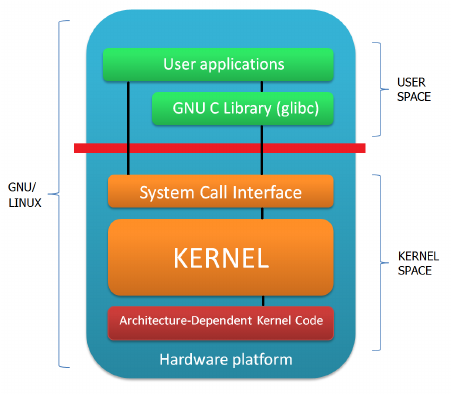
\includegraphics[width=0.6\textwidth]{pic_12}
\end{center}

В пространстве ядра работает, как не удивительно, само ядро ОС, а так же его модули (которые могут быть встроены в основное ядро, или могут быть представлены файлами в rootfs с расширением ko).

Пользовательские приложения и библиотеки работают в пользовательском пространстве. 

Ядро ОС Linux умеет работать с подгружаемыми модулями (если эта опция была активирована при сборке ядра). В качестве отдельных модулей могут выступать как определённые сервисы, предоставляемые ядром, так и драйверы устройств.

В Linux выделяют три типа устройств:
\begin{itemize}
	\item символьное устройство — представлено в файловой системой, минимальный объём данных один символ (или байт), примеры: клавиатура, мышь, принтер, тачскрин, экран, камера, spi устройство, i2c устройство и т.д. 
	\item блочное устройство — представлено в файловой системе, минимальный объём это блок данных, работа ведётся путём монтирования устройства. Примеры: карты памяти, SD карты и пр.  
	\item пакетное устройство — не представлено в файловой системе, устройство для взаимодействия пакетами, примеры: сетевой интерфейс, Wi-Fi, Bluetooth и т.д. 
\end{itemize}

В данной работе, мы создадим шаблон для символьного устройства, с которым можно будет взаимодействовать через пользовательское приложение.

\section{Сборка модуля}

\subsection{}Запустите виртуальную машину. Логин и пароль для входа: student / usrstudent.

\subsection{}Подключите по USB плату к ПК. Проверьте, и при необходимости подключите USB устройство FTDI RBM\_C1K5500VK018 к виртуальной машине (меню Device→USB).

\subsection{}Откройте консоль комбинацией клавиш Ctrl+Alt+T

\subsection{}Создайте рабочий каталог
\begin{lstlisting}[style=bash]
# mkdir -p $BAGET/lab_03 
\end{lstlisting}

\subsection{}Скопируйте в него рабочие файлы
\begin{lstlisting}[style=bash]
# cp -r $BAGET/support/mychar $BAGET/lab_03/
\end{lstlisting}

\subsection{}Перейдите в рабочий каталог и запустите vscode
\begin{lstlisting}[style=bash]
# cd $BAGET/lab_03/mychar; code .
\end{lstlisting}

\textbf{Замечание:} При первом входе, Вас могут спросить, доверяете ли вы автору, нужно нажать на кнопку Yes,  

\begin{center}
	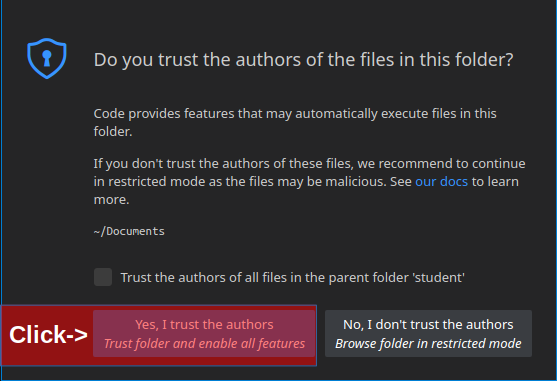
\includegraphics[width=0.6\textwidth]{pic_13}
\end{center}

\subsection{}Добавим путей для разрешения части include директив. Откройте .vscode -> c\_cpp\_properties.json
\begin{center}
	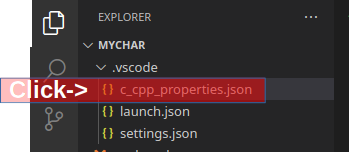
\includegraphics[width=0.6\textwidth]{pic_14}
\end{center}

\subsection{}Допишите в поле includePath следующие строки:\\
\begin{center}
	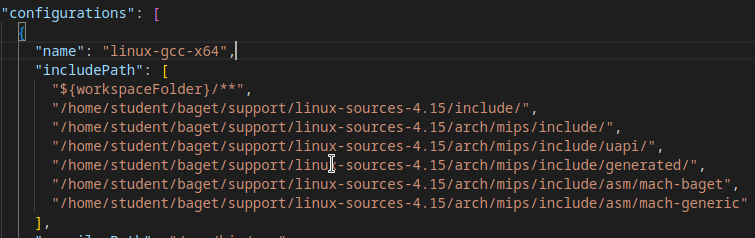
\includegraphics[width=\textwidth]{pic_15}
\end{center}
для удобства, воспользуйтесь файлом vscode\_lines.md в папке support.

Ctrl+S для сохранения

\subsection{}Откройте Makefile. Разберём основные моменты

obj-m  - тут мы задаём имя объектного файла верхнего уровня (файла из которого по итогу будет собран модуль). 

chardev-y — описываем, из каких объектных файлов будет собираться итоговый. 

KERNEL\_SRC — тут мы создаём переменную, которая будет хранить путь к заголовочным файлам ядра.

SRC — в этой переменной мы записываем путь к исходникам модуля, через вызов утилиты pwd. Таким образом, можно рабочую папку переносить куда угодно, без ручных правок. При сборке модуля, текущий путь меняется на путь KERNEL\_SRC, поэтому путь к исходникам модуля ядра должен быть абослютным.

all: — список команд выполняемых при сборке 

clean: — список команд выполняемых при очистке

\subsection{}Посмотрите на содержимое файла mychar\_init.c. Разберём основные моменты

В данном файле содержится минимальный набор кода, необходимый для сборки модуля ядра, и для его функционирования в системе. Нужно помнить, что данный код выполняется в пространстве ядра (Kernel space), соответственно не все парадигмы и функции привычные по работе с приложениями тут будут работать, хотя большинство из них имеют тут аналоги.

Обратите внимание на структур в районе 36 строки. Эта структура считывается ядром, при обращении к модулю, для установления связи между командами, отправляемыми через системный интерфейс, и функциями, которые их будут исполнять. Таким образом, достигается возможность исключить коллизий при работе с группой различных ядер. По той же причини, все структуры и функции объявлены с ключевым словом static.

Следующий момент, это структура объявляемая со строки 25. Параметр .compatible используется ядром, при сканировании дерева устройств. И при наличии совпадения, автоматически загружает модуль ядра.  


\subsection{}Посмотрите на содержимое файла mychar\_dev.c. В этом фале описан процесс инициализации символьного устройства, а так же работа с основными операциями (открытие файла, закрытие файла, считывание и запись данных).
Обратите внимание на функции работы с данными (srisa\_pdrv\_read и srisa\_pdrv\_write), для обмена данными между user space и kernel space используются специальные функции copy\_to\_user и copy\_from\_user.

\subsection{}Если кликать мышкой на вызываемую функцию, при зажатой клавише Ctrl, то редактор откроет вам реализацию этой функции в отдельной вкладке (если реализация находиться в другом файле). Попробуйте, так как далее Вам этот функционал понадобиться, при выполнении самостоятельных работ.

\subsection{}Перейдём в терминал (можно открыть вкладку TERMINAL в vscode, если её не видно, выберите в меню Terminal -> New Terminal) и соберём модуль командой
\begin{lstlisting}[style=bash]
# ARCH=mips CROSS_COMPILE=mips64el-linux-gnuabi64- make
\end{lstlisting}

\subsection{}Вы должны получить следующий вывод
\begin{center}
	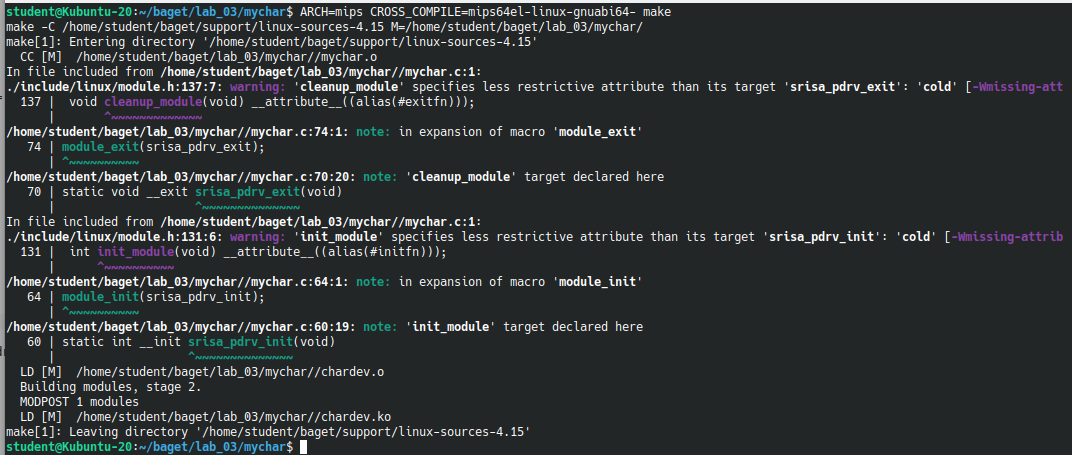
\includegraphics[width=\textwidth]{pic_16}
\end{center}
A в рабочей папке должны появиться несколько файлов, в том числе chardev.ko

\section{Настройка платы}
Для работы с модулями в Linux есть ряд команд

\textbf{insmod <path\_to\_module>} - подключение модуля ядра, с явным указанием пути к файлу, при этом не проверяются зависимости (бывает что один модуль требует предварительного запуска другого модуля).

\textbf{modporbe <module\_name>} - это «умная» версия insmod, проверяет зависимости (файл modules.dep), и подгружает их при необходимости. Не требуется указывать полный путь к модулю, однако модуль должен находиться в папке  /lib/modules/<kernel\_version>/

\textbf{lsmod} — выводит список активированных модулей, с указанием счётчика зависимостей (показывает сколько потоков использует данный модуль)

\textbf{rmmod <module\_name>} - выгрузить указанный модуль (указывается только имя модуля, без расширения ko)

\subsection{}Откройте gtkterm и подключитесь к плате (/dev/ttyUSB1 скорость 115200)

\subsection{}Создадим каталог, для нормальной работы утилиты modporbe. Для этого выполните команду
\begin{lstlisting}[style=bash]
$ mkdir -p /lib/modules/$(uname -r)/
\end{lstlisting}

\subsection{}Создадим два пустых файла
\begin{lstlisting}[style=bash]
$ touch  /lib/modules/$(uname -r)/modules.order
$ touch  /lib/modules/$(uname -r)/modules.builtin
\end{lstlisting}
В данном случае, допустим такой ход, но в общем случае, содержимое этих файлов должно отражать реальность.

\subsection{}Вернёмся в консоль виртуальной машины, и скопируем скомпилированный модуль на плату (проверьте, что плата подключена сетевым шнуром к рабочему ПК)
\begin{lstlisting}[style=bash]
# scp $BAGET/lab_03/mychar/chardev.ko \
netuser@192.168.100.200:/home/netuser/
\end{lstlisting}
пароль - usrnetuser

\subsection{}Вернитесь в терминал платы, и скопируйте ядро
\begin{lstlisting}[style=bash]
$ cp /home/netuser/chardev.ko /lib/modules/$(uname -r)/
\end{lstlisting}

\subsection{}Определим зависимости для модуля, для чего выполните команду 
\begin{lstlisting}[style=bash]
$ depmod
\end{lstlisting}
Данная команда просканирует все модули, в папке /lib/modules/\$(uname -r)/ и запишет о них информацию. После чего модули могут подгружаться командой modprobe. 

\subsection{}Проверим работу нашего модуля, выполнив команду
\begin{lstlisting}[style=bash]
$ modprobe chardev
\end{lstlisting}
Вы должны увидеть надпись 
\begin{lstlisting}[style=stdout]
srisa_pdrv: srisa_pdrv_init
\end{lstlisting}

\subsection{}Просмотрим список загруженных модулей
\begin{lstlisting}[style=bash]
$ lsmod
\end{lstlisting}
Вы должны увидеть надпись 
\begin{lstlisting}[style=stdout]
Module                  Size  Used by
chardev                 4620  0
\end{lstlisting}
Как мы видим, никто не использует наше ядро (Used by равен 0). 

\subsection{}Выполните команду ls /dev/* Обратите внимание, что отсутствует файл srisa\_pdrv, так как он создаётся, только при вызове функции pdrv\_probe, вызываемая только при наличии совместимого периферийного модуля.

\subsection{}Выгрузим из памяти наше ядро
\begin{lstlisting}[style=bash]
$ rmmod chardev
\end{lstlisting}

\section{Правка дерева устройств (device-tree)}
Мы успешно собрали модуль устройства, однако его сейчас никто не использует. Как говорилось выше, часто модули ядра являются драйвером, для взаимодействия с периферией (как внутрипроцессорной, типа интерфейса spi, так и внешней). Для описания взаимодействия между ядром я устройством служит специальная структура дерево устройств (device tree). В ней описывается основная информация о устройстве, а так же могут добавлять параметры, применяемые модулем ядра, при работе с тем или иным устройством. Среди прочего, дерево устройств поддерживает функцию перезаписи, что позволяет создавать мелкие файлы, вносящие исправление в существующее описание, или дополняющее его, в соответствии с требованиями конкретного проекта.

\subsection{}Создадим рабочую папку в виртуальной машине для дополнения дерева устройств и перейдём в неё
\begin{lstlisting}[style=bash]
# mkdir $BAGET/lab_03/devtree
# cd $BAGET/lab_03/devtree 
\end{lstlisting}

\subsection{}Создадим файл и откроем его для редактирования
\begin{lstlisting}[style=bash]
# kate of_mychard.dts
\end{lstlisting}

\subsection{}Запишите в файл следующие строки
\begin{lstlisting}[style=stdout]
/dts-v1/;

/ {
	fragment@0 {
		target-path = "/";
		__overlay__ {
			
			pdrv1 {
				compatible = "srisa,platform-device";
				status = "okay";
			};
		};
	};
};
\end{lstlisting}

\subsection{}Сохраните Ctrl+S и закройте редактор Ctrl+Q

Мы создали дополнение, которое описывает виртуальное устройство, совместимое с драйвером, который мы создали ранее (обратите внимание на поле compatible в написанном фрагменте, и сравните его значение со значением одноименного параметра в исходном коде модуля). 

\subsection{}Скомпилируем дополнение к дереву устройств, для этого выполним следующую команду
\begin{lstlisting}[style=bash]
# dtc -@ -O dtb -o ./of_mychard.dtb ./of_mychard.dts
\end{lstlisting}

\vspace{5mm}
Если у Вас есть уже скомпилированное дерево устройств, Вы можете вернуть его в «человеческий вид» командой 
\begin{lstlisting}[style=bash]
# dtc --symbol -O dts -o ./out.dts ./source.dtb
\end{lstlisting}

\subsection{}Скопируйте полученный файл на плату
\begin{lstlisting}[style=bash]
# scp $BAGET/lab_03/devtree/of_mychard.dtb \
netuser@192.168.100.200:/home/netuser/
\end{lstlisting}

\subsection{}Перейдите в терминал платы, и переместите скопированный файл в папку barebox
\begin{lstlisting}[style=bash]
$ mv /home/netuser/of_mychard.dtb /barebox/
\end{lstlisting}

\subsection{}Отредактируйте скрипт barebox.sh
\begin{lstlisting}[style=bash]
$ nano /barebox/barebox.sh
\end{lstlisting}
и впишите в него, после строки DTB=k5500vk018\_rbm.dtb
\begin{lstlisting}[style=stdout]
fdt_apply -i $DTB -l of_mychard.dtb -o /dtb && DTB=/dtb
\end{lstlisting}
Ctrl+S, Ctrl+X 

\subsection{}Перезагрузите плату командой reboot

\section{Проверка работы модуля}

\subsection{}Войдите как пользователь root, и выполните команду lsmod.
Модуль должен быть уже загружен, так как ядро при запуске должно было обнаружить в дереве устройств, совместимое с нашим модулем. 

\subsection{}Посмотрим последние строки лога загрузки ядра
\begin{lstlisting}[style=bash]
$ dmesg | tail
\end{lstlisting}
Вы должны увидеть следующие строки в выводе
\begin{lstlisting}[style=stdout]
...
[ 27.263923] srisa_pdrv: srisa_pdrv_init
[ 27.266836] srisa_pdrv: pdrv_probe
...
\end{lstlisting}

Строку с init мы видели ранее, но теперь после неё есть строка srisa-pdrv: pdrv\_probe, которая говорит нам, что наш модуль успешно связался с устройством описанным нами в дополнении к дереву устройств.

\subsection{}Выполните команду ls /dev/* и обратите внимание, что должен появиться файл srisa\_pdrv.

\subsection{}Отправим данные в srisa\_pdrv, и проверьте ответ
\begin{lstlisting}[style=bash]
$ echo 1234 > /dev/srisa_pdrv
\end{lstlisting}
\begin{lstlisting}[style=stdout]
srisa_pdrv: srisa_pdrv_open
srisa_pdrv: srisa_pdrv_ioctl
srisa_pdrv: srisa_pdrv_write: Get 5 bytes
srisa_pdrv: srisa_pdrv_release
\end{lstlisting}
Замечание: принято пять байт, так как последний байт это байт перевода каретки (\textbackslash{}r). 

\subsection{}Посмотрим на скорость записи данных, для этого выполните команду:
\begin{lstlisting}[style=bash]
$ dd count=1 bs=1M if=/dev/zero of=/dev/srisa_pdrv 
\end{lstlisting}
Команда dd может часто встречаться Вам при активной работе с Linux. Она обеспечивает считывание, или копирование данных из одного файла в другой. В данном случае, мы указываем, что ходим один раз (count=1) отправить 1 мегабайт (bs=1M)  из файла /dev/zero (генератор 0) в наш драйвер. Чем больше мы отправим данных, тем точнее получим значение скорости, однако из-за особенностей реализации считывания в нашем драйвере, большой объём данных может привести к печальным последствиям, так что увлекаться не стоит. Результат должен быть таким
\begin{lstlisting}[style=stdout]
srisa_pdrv: srisa_pdrv_open
srisa_pdrv: srisa_pdrv_write: Get 1048576 bytes
srisa_pdrv: srisa_pdrv_release 
1+0 records in
1+0 records out
1048576 bytes (1.0 MB, 1.0 MiB) copied, 0.0318856 s, 32.9 MB/s
\end{lstlisting}
Последняя строка показывает сколько данных было передано, и на какой скорости. Результат может менятся от каждого запуска, но порядок величин должен быть одинаковый.

\subsection{}Попробуем считать данные из драйвера, для этого выполним следующую команду: 
\begin{lstlisting}[style=bash]
$ dd count=1 bs=10 if=/dev/srisa_pdrv
\end{lstlisting}
Тут мы опять используем команду dd, но на этот раз не указываем выходной файл, поэтому сможем увидеть вывод в консоли
\begin{lstlisting}[style=stdout]
srisa_pdrv: srisa_pdrv_open 
srisa_pdrv: srisa_pdrv_read: Send 10 bytes 
ABCDEFGHIsrisa_pdrv: srisa_pdrv_release 
1+0 records in 
1+0 records out 
10 bytes copied, 0.0131135 s, 0.8 kB/s
\end{lstlisting}
Как видите, в выводе мы увидели набор букв, который был сгенерирован нашим драйвером.  

\subsection{}Измерим скорость чтения данных, но на этот раз перенаправим вывод в файл: 
\begin{lstlisting}[style=bash]
$ dd count=1 bs=1M if=/dev/srisa_pdrv of=/root/drv.out
\end{lstlisting}
\begin{lstlisting}[style=stdout]
srisa_pdrv: srisa_pdrv_open 
srisa_pdrv: srisa_pdrv_read: Send 1048576 bytes 
srisa_pdrv: srisa_pdrv_release 
1+0 records in 
1+0 records out 
1048576 bytes (1.0 MB, 1.0 MiB) copied, 0.140926 s, 7.4 MB/s
\end{lstlisting}
Скорость на чтение меньше, чем на запись, так как драйвер в начале заполняет свой внутренний массив, и затем отправляет данные. Так же тормозит и запись файла. Проверьте это, заменив файл назначения на /dev/null Для просмотра вывода выполните команду cat /root/drv.out и немного подождём, пока через терминал будет передан 1 мегабайт алфавита. Вывод можно прервать комбинацией Ctrl+C

\subsection{}Выгрузим ядро 
\begin{lstlisting}[style=bash]
$ rmmod chardev
\end{lstlisting}
И снова мы видим, что есть два вывода, один от модуля, который видели ранее, второй сообщает нам, что была выполнена функция по отключению от устройства.  

\subsection{}Введите команду poweroff, дождитесь, пока не появиться надпись: reboot: System halt, после чего отключите USB кабель от ПК. 

\section{Задание для закрепления}
Внесите правки в модуль ядра, так, что бы командой считывания можно было получить все данные, записанные ранее через команду записи. Другими словами, пользователь два раза записал Hello после чего запросил на считывание 1Мбайт, в ответ он должен получить 10 байт: HelloHello.

Замечание: тут нам понадобиться работа со структурой kfifo (в коде переменная data\_fifo). В коде уже вставлены части по её инициализации (mychar\_dev.c), Вам остаётся вписать в нужные места вызовы функций для считывания и записи данных. При этом функция copy\_from\_user и copy\_to\_user уже не нужны.

Командой dd можно передавать данные из любых файлов, что может помочь Вам в проверке работы драйвера. Как один из вариантов, Вы создаёте текстовый файл, и пишите в него текст, далее, через комманду dd передаёте в драйвер, и второй командой dd считываете данные в другой файл, после чего можете сравнить два файла коммандой diff <path1> <path2>

Пример для записи данных в драйвере.
\begin{lstlisting}[style=stdout]
static ssize_t fifo_write(struct file *file, const char __user *buf, size_t count, loff_t *ppos)
{
	int ret;
	unsigned int copied;
	
	ret = kfifo_from_user(&test, buf, count, &copied);
	
	return ret ? ret : copied;
}
\end{lstlisting}


Пример для считывания данных из драйвера.
\begin{lstlisting}[style=stdout]
static ssize_t fifo_read(struct file *file, char __user *buf, size_t count, loff_t *ppos)
{
	int ret;
	unsigned int copied;
	
	ret = kfifo_to_user(&test, buf, count, &copied);
	
	return ret ? ret : copied;
}
\end{lstlisting}

\subsubsection{*} Модифицировать код таким образом, что бы  можно было независимо обрабатывать два устройства (для проверки добавьте в device tree ещё одно устройство, pdrv2)

	%\chapter{Драйвер GPIO}
\textbf{Цель:} Управление выводами через встроенные в ядро драйверы и написание своего драйвера, для работы с выводами.

\vspace{5mm}
\textbf{Описание:}В предыдущей работе мы узнали, как можно управлять выводами через виртуальную файловую систему sysfs. Однако, при работе с внешними модулями, помимо интерфейса для передачи данных, могут понадобиться выводы, для управления состоянием модуля (сигнал сброса), или для проверки события (вывод ALARM на некоторых промышленных устройствах). Так же нам могут понадобиться выводы для индикации, или ввода информации. В этой работе Вы узнаете, как можно работать с выводами общего назначения через стандартные драйверы ядра, и как ими пользоваться в своих драйверах. 

\vspace{5mm}
\textbf{Полезные ссылки:}
\begin{itemize}
	\item \href{https://www.kernel.org/doc/Documentation/devicetree/bindings/input/gpio-keys.txt}{Kernel Doc: GPIO Keys}.
	\item \href{https://www.kernel.org/doc/Documentation/devicetree/bindings/leds/common.yaml}{Kernel Doc: LED's Common}.
	\item \href{https://docs.kernel.org/devicetree/dynamic-resolution-notes.html}{Kernel Doc: Devicetree Dynamic Resolver Notes}
	\item \href{https://www.kernel.org/doc/html/v4.15/driver-api/gpio.html}{Kernel Doc: General Purpose Input/Output (GPIO)}
	\item \href{https://git.kernel.org/pub/scm/linux/kernel/git/torvalds/linux.git/tree/include/uapi/linux/input-event-codes.h}{Kernel GIT: Input Event Codes}
	\item \href{https://www.kernel.org/doc/Documentation/gpio/consumer.txt}{Kernel Doc: GPIO Descriptor Consumer Interface}	
\end{itemize}

\section{Встроенные драйверы}
Наверное, одно из самые распространённые способы использования выводов общего назначения (GPIO) для считывания состояния кнопок (клавиатура, мышь, кнопка сброса и выключения), и простейшей индикации средствами светодиодов (доступ к диску,  индикация наличия питания, активации режима Caps Lock и пр.). В ядре Linux есть готовые драйверы для использования GPIO как кнопок или индикаторов. В данном разделе, мы с Вами посмотрим, как можно управлять выводами общего назначения через эти драйверы.

\subsection{}Запустите виртуальную машину. Логин и пароль для входа: student / usrstudent.

\subsection{}Подключите по USB плату к ПК. Проверьте, и при необходимости подключите USB устройство FTDI RBM\_C1K5500VK018 к виртуальной машине (меню Device→USB).

\subsection{}Откроете терминал комбинацией клавиш Ctrl+Alt+T

\subsection{}Для начала подготовим рабочую папку, для разработки дополнения к дереву устройств системы: 
\begin{lstlisting}[style=bash]
# mkdir -p $BAGET/lab_04/of_dtb/
# cd $BAGET/lab_04/of_dtb/
\end{lstlisting}

\subsection{}Создадим и приступим к правке дополнения 
\begin{lstlisting}[style=bash]
# kate ./of_gpio.dts
\end{lstlisting}

\subsection{}Впишите следующие строки
\begin{lstlisting}[style=stdout]
/dts-v1/;
/plugin/;
/ {
	fragment@0 {
		target-path = "/";
		__overlay__ {
			grnled {
				compatible = "gpio-leds";
				led1 {
					label = "led1";
					gpios = <&gpiof 0 0>;
					linux,default-trigger = "heartbeat";
					default-state = "off";
				};
			};
			
			button {
				compatible = "gpio-keys";
				status = "okay";
				#address-cells = <1>;
				#size-cells = <0>;
				autorepeat;
				btn {
					label = "btn";
					linux,code = <4>;
					gpios = <&gpiod 6 1>;
				};
			};
		};
	};
};
\end{lstlisting}

Первая часть, отвечает за передачу управления светодиодом, подключённому к выводу F0, драйверу gpio-leds. Данный драйвер позволяет не только включать и выключать светодиод, но и активизировать его, при срабатывании одного из триггеров. К сожалению в текуще сборки ядра триггеры не были активированы (каждый триггер по сути это отдельный модуль ядра), поэтом мы не сможем посмотреть их в действии.

Вторая часть отвечает за настройку кнопки. В данном случае, при нажатии кнопки будет формироваться событие отправки символа Q (код кнопки 16). Полный список кодов кнопок можно посмотреть в файле по ссылке 5 в начале лабораторной работы.

Параметр gpios определяет, какой вывод мы отдаём под управление драйвером. Входное значение представления из себя массив из трёх элементов:
\begin{enumerate}
	\item ссылка на банк выводов,
	\item номер вывода в указанном банке,
	\item полярность сигнала (0 — прямая, 1 — инверсная)
\end{enumerate}

\subsection{}Сохраните файл Ctrl+S и закройте редактор Ctrl+Q

\subsection{}Скомпилируем наш фрагмент, для этого выполним следующую команду 
\begin{lstlisting}[style=bash]
# dtc --symbol -O dtb -o ./of_gpio.dtb ./of_gpio.dts
\end{lstlisting}
Замечание: при компиляции будет выдано предупреждение, его можно проигнорировать.

\subsection{}Скопируйте полученный файл на плату
\begin{lstlisting}[style=bash]
# scp ./of_gpio.dtb netuser@192.168.100.200:/home/netuser/
\end{lstlisting}

\subsection{}Откройте программу gtkterm, и подключитесь к порту /dev/ttyUSB1

\subsection{}Переместите скопированный файл в папку barebox
\begin{lstlisting}[style=bash]
$ mv /home/netuser/*.dtb /barebox/
\end{lstlisting}

\subsection{}Откройте скрипт barebox.sh для редактирования
\begin{lstlisting}[style=bash]
$ nano /barebox/barebox.sh
\end{lstlisting}

\subsection{}Впишите после строки DTB=k5500vk018\_rbm.dtb следующую строчку 
\begin{lstlisting}[style=stdout]
fdt_apply -i $DTB -l ./of_gpio.dtb -o /dtb && DTB=/dtb
\end{lstlisting}
при наличии строки от прошлых работ, можно её переписать, удалить или оставить.

Сохраним изменения и выйдем из редактора: Ctl+S,  Ctrl+X

\subsection{}Перезагрузите плату командой reboot, и внимательно изучите лог загрузки.

После того, как отработает отключение системы (записи, начинающиеся с [ OK ]). Система начнёт загрузку. Найдите в логе такие строки:
\begin{lstlisting}[style=stdout] 
Hit m for menu or any other key to stop autoboot: 0
Booting entry 'mmc'
ext4 ext40: EXT2 rev 1, inode_size 256, descriptor size 32
eth1.ethaddr is not set
add_eth_mac_addr() failed for eth1 (1)
Skip dumping CK64 regs values to overlay: target CPU \freq 0 is less than or equal to 400000000
Entry Point: ffffffff807d5cd0
\end{lstlisting}
Если у Вас вывод не совпадает с выводом выше, то скорее всего Вы допустили ошибку в dts файле. Проверьте, что Вы правильно записали текст исправления дерева устройств.

\section{Проверка}

\subsection{}Посмотрим на работу кнопки, для чего воспользуемся специальной утилитой для анализа событий
\begin{lstlisting}[style=bash]
$ evtest /dev/input/event0  
\end{lstlisting}
Как только вы её запустите, то увидите информацию о проверяемом источнике ввода:
\begin{center}
	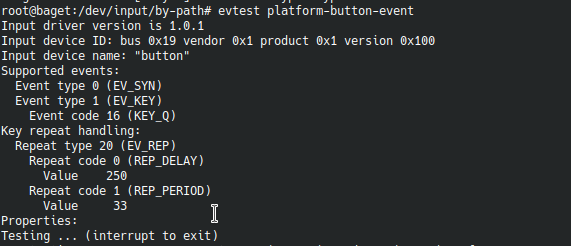
\includegraphics[width=\textwidth]{pic_17}
\end{center}

\subsection{}Нажмите и отпустите кнопку. Вы увидите как в консоли появиться несколько записей. Это информация о событии. 
\begin{center}
	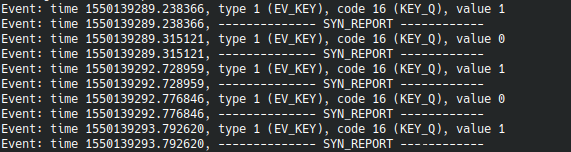
\includegraphics[width=\textwidth]{pic_18}
\end{center}
Замечание: обратите внимание на значение параметра value, оно кодирует состояние кнопки 0 — отпущена, 1 — нажата, 2 — удерживается  

\subsection{}Прервём работу команды, нажав Ctrl+C (рекомендуется её запомнить, при работе с консолью в Linux, эта комбинация используется часто, для прерывания выполнения текущей команды или программы)

\subsection{}Дополнительно посмотрим, что на самом деле считывается из файла при работе с ним, для чего запустим конвейер из двух команд
\begin{lstlisting}[style=bash]
$ cat /dev/input/event0 | hexdump 
\end{lstlisting}
Тут уже при открытии Вы не увидите ничего, однако как только начнёте нажимать и отпускать кнопку, то увидите поток данных. В этом потоке храниться как информация о событии, так и временные метки, что мы видели ранее, инструмент evtest занимается преобразованием (парсингом) этого потока, в человечески воспринимаемый вид. 

\subsection{}Прервём работу нажав Ctrl+C.

\subsection{}Светодиоды управляются через виртуальную файловую систему sysfs. Перейдите в следующий каталог
\begin{lstlisting}[style=bash]
$ cd /sys/class/leds
\end{lstlisting}

\subsection{}Тут располагаются ссылки на все светодиоды доступные в системе. В нашем случае, дожно быть две папки mmc0:: и led1, проверьте выполнив команду  
\begin{lstlisting}[style=bash]
$ ls -l
\end{lstlisting}

\subsection{}Для управления состоянием светодиода отправьте 1 в файл brightness для включения светодиода, и 0 для выключения. При подключении через ШИМ контроллер, этот файл позволяет устанавливать яркость светодиода (например, для управления яркостью подсветки экрана)
\begin{lstlisting}[style=bash]
$ echo 1 > led1/brightness
$ echo 0 > led1/brightness
\end{lstlisting}

\section{Собираем свой драйвер}
Попробуем теперь использовать вывод общего назначения внутри собственного драйвера, что может часто понадобиться, при работе с внешними модулями. К примеру, для управления сигнала сброса, или для переключения между режимами и т. д.

\subsection{}Скопируем код демонстрирующий работу с GPIO в пространстве ядра. Вернитесь в консоль виртуальной машины, и выполните следующую команду, и посмотрим в него 
\begin{lstlisting}[style=bash]
# cp -r $BAGET/support/gpio_driver $BAGET/lab_04/driver
# cd $BAGET/lab_04/driver; code .
\end{lstlisting}
\begin{center}
	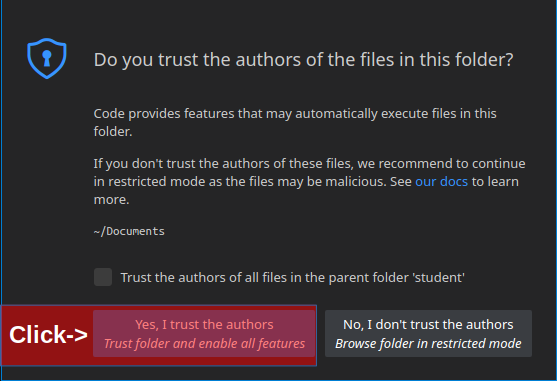
\includegraphics[width=\textwidth]{pic_13}
\end{center}
\textbf{Замечание:} При первом входе, Вас могут спросить, доверяете ли вы автору, нужно нажать на кнопку Yes,  


\subsection{}Добавим путей для разрешения части include директив. Откройте .vscode -> c\_cpp\_properties.json
\begin{center}
	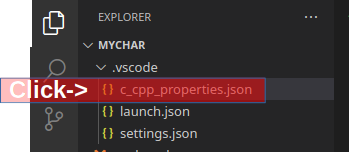
\includegraphics[width=\textwidth]{pic_14}
\end{center}

\subsection{}Допишите в поле includePath следующие строки:\\
\begin{center}
	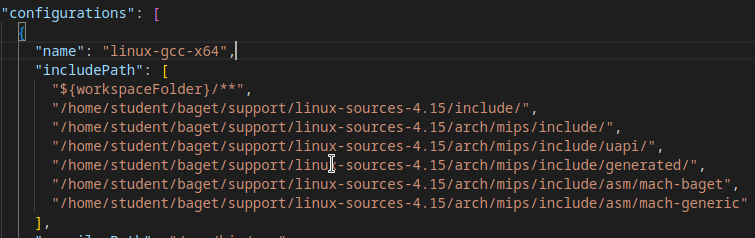
\includegraphics[width=\textwidth]{pic_15}
\end{center}
для удобства, воспользуйтесь файлом vscode\_lines.md в папке support.

Ctrl+S для сохранения.

\subsection{}Допишем compilerArgs, как на картинке ниже, для корректного перехода к реализации функций gpio драйвера ядра.\\
\begin{center}
	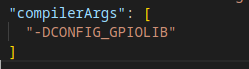
\includegraphics[width=0.5\textwidth]{pic_19}
\end{center}

\subsection{}Посмотрим на содержимое файла gpio\_temp.c. В нём описан процесс подключения драйвера к выводу.

\subsection{}Так же откройте, и посмотрите на Makefile. В нём есть раздел install который поможет Вам скопировать на целевую плату скомпилированный модуль ядра. При этом, перед копированием будет запущена сборка всего проекта. Это полезная практика, так как гарантирует Вам, что при исправлении мелкой опечатки, на плату попадёт код с исправлением, а не его предыдущая версия.

\subsection{}Перейдём в терминал (можно открыть вкладку TERMINAL в vscode, если её не видно, выберите в меню Terminal → New Terminal) и соберём модуль командой:
\begin{lstlisting}[style=bash]
# ARCH=mips CROSS_COMPILE=mips64el-linux-gnuabi64- make 
\end{lstlisting}

\subsection{}Проверьте значение системной переменной BRD\_PASS  
\begin{lstlisting}[style=bash]
# echo $BRD_PASS
\end{lstlisting}
если вывод был пустой, проинициализируйте переменную 
\begin{lstlisting}[style=bash]
# export BRD_PASS="usrnetuser" 
\end{lstlisting}
и скопируйте модуль на плату
\begin{lstlisting}[style=bash]
# ARCH=mips CROSS_COMPILE=mips64el-linux-gnuabi64- make install
\end{lstlisting}
Замечание: попробуйте сами разобратся, как в Makefile описан процес копирования файла на плату. Это может Вам помочь, при выполнении самостоятельных работ.

\subsection{}Внесите изменения в файл дерева-устройств 
\begin{lstlisting}[style=bash]
# kate $BAGET/lab_04/of_dtb/of_gpio.dts
\end{lstlisting}
удалите ноды led1 и button, и допишите новую ноду:
\begin{lstlisting}[style=stdout]
custom {
	compatible = "gpio,dummy";
	status = "okay";
	yellowled-gpios = <&gpiof 1 0>;
};
\end{lstlisting}
Замечание: обратите внимание на строку, в которой мы указываем информацию о выводе, которым нужно управлять. Первая часть (yellowled…) должна совпадать с той меткой, что указана в исходном коде, на 62 строке!

\subsection{}Сохраните изменения Ctrl+S и закройте редактор Ctrl+Q 

\subsection{}Скомпилируем файл dts, для этого выполним следующую команду
\begin{lstlisting}[style=bash]
# dtc --symbol -O dtb -o $BAGET/lab_04/of_dtb/of_gpio.dtb \
$BAGET/lab_04/of_dtb/of_gpio.dts
\end{lstlisting}

\subsection{}Скопируйте полученный файл на плату
\begin{lstlisting}[style=bash]
# scp $BAGET/lab_04/of_dtb/of_gpio.dtb \
netuser@192.168.100.200:/home/netuser/
\end{lstlisting}

\subsection{}Перейдите в терминал платы, и переместите файл в папку barebox
\begin{lstlisting}[style=bash]
$ mv /home/netuser/*.dtb /barebox/
\end{lstlisting}

\subsection{}Перезагрузите плату командой reboot

\subsection{}После перезагрузки, подгрузите модуль командой
\begin{lstlisting}[style=bash]
$ insmod /home/netuser/gpio_temp.ko
\end{lstlisting}
Если не было допущено ошибок, то в течении 20 секунд плата будет перемигиваться с Вами светодиодами F0 и F1

\section{Задание для закрепления}
Измените код таким образом, что бы светодиод начинал мигать, когда кнопка нажата. Для этого воспользуйтесь таймером.

\begin{itemize}
	\item Добавьте функцию инициализирующую кнопку (нужно сделать всё то же, что и при инициализации светодиода, в функции int myled\_init(int gpio\_id), за исключением того, что направления вывода должно быть GPIOD\_INPUT
	
	\item Для считывания состояния кнопки, используйте функцию gpio\_get\_value(<gpio\_id>). Помните, что кнопка на плате имеет инверсную логику, другими словами в отпущенном состоянии вывод прижат к питанию, и возвращает 1.
	
	\item Пример кода по инициализации таймера
	\begin{lstlisting}[style=stdout]
		      #include <linux/module.h> /* Needed by all modules */
		#include <linux/kernel.h> /* Needed for KERN_INFO */
		#include <linux/init.h> /* Needed for the macros */
		#include <linux/timer.h>
		#include <linux/jiffies.h>
		
		int g_time_interval = 250; // miliseconds
		struct timer_list g_timer;
		
		void _TimerHandler(struct timer_list *tm)
		{
			static bool state = true;
			printk("%s: %s", DRIVER_NAME, __func__);
			state = !state;
			mod_timer(tm, jiffies + msecs_to_jiffies(g_time_interval));
		}
		
		static int __init my_init(void)
		{
			printk(KERN_INFO "My module inserted into kernel!!!.\n");
			
			/*Starting the timer.*/
			setup_timer(&g_timer, _TimerHandler, 0);
			mod_timer( &g_timer, jiffies + msecs_to_jiffies(g_time_interval));
			
			return 0;
		}
		
		static void __exit my_exit(void)
		{
			del_timer(&g_timer);
			printk(KERN_INFO "My module exited from kernel!!!\n");
		}
		
		module_init(my_init);
		module_exit(my_exit);
	\end{lstlisting}

	\item не забудьте добавить освобождение ресурсов для кнопки и таймера.
\end{itemize}
	%\chapter{Драйвер SPI устройства}
\textbf{Цель:} Активировать SPI контроллер, и написать простой драйвер для устройства подключённого к SPI интерфейсу.

\vspace{5mm}
\textbf{Описание:}В данной работе, мы познакомимся со структурой ядра, позволяющей взаимодействовать с spi контроллером целевой платы. Данная структура является программным интерфейсом, позволяющим отвязать реализацию взаимодействия с внешним аппаратным модулем по интерфейсу SPI, от особенностей реализации SPI контроллера на конкретной аппаратной платформе. 

\vspace{5mm}
\textbf{Полезные ссылки:}
\begin{itemize}
	\item \href{http://www.gaw.ru/html.cgi/txt/interface/spi/index.htm}{Последовательный интерфейс SPI}.
	\item \href{https://docs.kernel.org/devicetree/dynamic-resolution-notes.html}{Kernel Doc: Devicetree Dynamic Resolver Notes}
	\item \href{https://www.kernel.org/doc/html/v4.15/driver-api/spi.html}{Kernel Doc: SPI API}	
\end{itemize}

\section{Запуск и подключение к устройству}

\subsection{}Запустите виртуальную машину. Логин и пароль для входа: student / usrstudent.

\subsection{}Подключите по USB плату к ПК. Проверьте, и при необходимости подключите USB устройство FTDI RBM\_C1K5500VK018 к виртуальной машине (меню Device→USB).

\subsection{}Откройте программу gtkterm, и подключитесь к порту /dev/ttyUSB1

\subsection{}Если в окне терминала нет текста, нажмите клавишу Enter на клавиатуре. Вы должны увидеть следующий вывод:
\begin{center}
	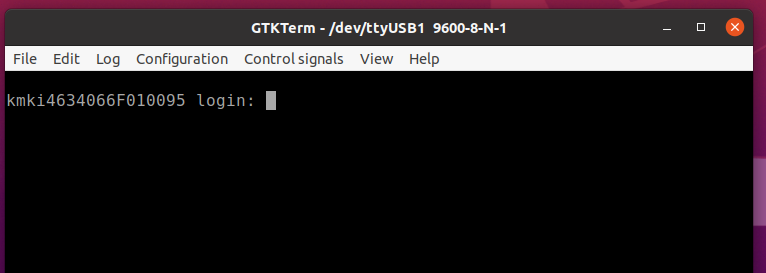
\includegraphics[width=\textwidth]{pic_08}
\end{center}
Вы подключились к консоли устройства. Введите логин root и пароль root.


\section{Подготовка Device Tree Overlay}
Основная конфигурация целевой платы предполагает, что практически все выводы настроены для управления через блок GPIO. Для работы с SPI, нам необходимо ввести две правки: разрешить работу SPI контроллера и передать под его управления выводы, для коммуникации с внешним миром. 

\subsection{} Создадим рабочую папку в виртуальной машине для создания device-tree overlay и перейдём в неё 
\begin{lstlisting}[style=bash]
# mkdir -p $BAGET/lab_05/devtree
# cd $BAGET/lab_05/devtree
\end{lstlisting}

\subsection{}Создадим новый файл
\begin{lstlisting}[style=bash]
# kate of_spi1.dts
\end{lstlisting}
и запишем в него следующий текст
\begin{lstlisting}[style=stdout]
/dts-v1/;
/plugin/;
/ {
	fragment@0 {
		target-path = "/gpio@1b400200";
		
		__overlay__ {
			
			spi1_pins {
				phandle = <0x01>;
				
				spi1_clk {
					function = "spi1_clk";
					groups = "spi1_clk";
				};
				
				spi1_di {
					function = "spi1_di";
					groups = "spi1_di";
				};
				
				spi1_do {
					function = "spi1_do";
					groups = "spi1_do";
				};
				
				spi1_cs0 {
					function = "spi1_cs0";
					groups = "spi1_cs0";
				};
			};
		};
	};
	
	
	fragment@1 { 
		target-path = "/spi@1a800000"; 
		
		__overlay__ { 
			status = "okay"; 
			pinctrl-names = "default"; 
			pinctrl-0 = <0x01>; 
		}; 
	}; 
	
	
	__local_fixups__ {
		
		fragment@1 {
			__overlay__ {
				pinctrl-0 = <0x00>;
			};
		};
		
	};
};
\end{lstlisting}

Разберём, что мы тут создали. Данное дополнение состоит из нескольких фрагментов, так как переписать нам нужно две разные ноды, однако изменения эти должны быть синхронизированы между собой, по этой причине они находятся в одном файле. 

Первый фрагмент, это дополнение к ноде описывающей банк выводов А. В этом дополнении мы создаём конфигурацию, для передачи управления частью выводов SPI контроллеру. Будьте внимательны, не любой вывод может быть передан SPI контроллеру. 

Следующий фрагмент правок, касается дополнения к описанию spi контроллера. Первое, это его активация, записью в параметр status значения okay. Так же, мы вводим два дополнительных параметра, один хранит в себе название конфигурации выводов, второй — для указания идентификатора конфигурации, обратите внимание, что значение у него совпадает (и это важно) со значением phandle у описания выводов из первого фрагмента.

Последняя строка гарантирует, что после применения этого дополнения, значение параметра pinctrl-0 будет соответствовать значению phandle нашей группы spi1\_pins. Дело в том, что значение phandle из первого фрагмента, будет  актуализировано, для разрешения коллизий (так как в исходном device-tree уже есть нода, с таким значением phandle), и последняя строка в нашем описании исправлений поясняет системе, что после разрешения коллизии, необходимо обновить значение указанного параметра (значение 0 зарезервировано, и в данном контексте означает ссылку на значение параметра phandle).  

Узнать, какой банк выводов, и какие выводы могут быть использованы с тем или иным интерфейсом, какие значения phandle уже использованы, и просто для любопытства можно одним из двух способов:

\begin{enumerate}
	\item Из самой системы, изучив подкаталоги gpio, в каталоге /proc/device-tree/ (рекомендуется для считывания значение того или иного параметра использовать команду cat). 
	
	\item Преобразовав бинарный файл device-tree системы в текстовый вид 
	\begin{lstlisting}[style=bash]
	# dtc --symbol -O -dts -o  /tmp/root.dts \
	$BAGET/support/barebox/k5500vk018_rbm.dts
	# kate /tmp/root.dts
	\end{lstlisting}
\end{enumerate}

Посмотрите на ноды, описывающие банки GPIO выводов. Так же обратите внимание, на объявление конфигураций выводов для sdhci контроллера, особенно, как эта конфигурация разбита, между двумя банками выводов, на значение параметра phandle каждой группы. Сравните значение параметров phandle конфигурационных груп, и значения перечисленные в параметре pinctrl-0 у ноды для контроллера  sdhci. (не стесняйтесь использовать поиск по файлу).

\subsection{}Сохраните изменения Ctrl+S и закройте редактор Ctrl+Q 

\subsection{}Скомпилируем файл и скопируем его на плату
\begin{lstlisting}[style=bash]
# dtc --symbol -O dtb -o ./of_spi1.dtb ./of_spi1.dts
# scp ./of_spi1.dtb netuser@192.168.100.200:/home/netuser/
\end{lstlisting}

\subsection{}Перейдите в терминал платы, и переместите файл в папку barebox
\begin{lstlisting}[style=bash]
$ mv /home/netuser/of_spi1.dtb /barebox/
\end{lstlisting}

\subsection{}Откройте скритп barebox.sh для редактирования
\begin{lstlisting}[style=bash]
$ nano /barebox/barebox.sh
\end{lstlisting}

\subsection{}Впишите после строки DTB=k5500vk018\_rbm.dtb следующую строчку (при наличии других строк, закомментируйте их символом \# )
\begin{lstlisting}[style=stdout]
fdt_apply -i $DTB -l of_spi1.dtb -o /dtb && DTB=/dtb
\end{lstlisting}
Сохраним изменения и выйдем из редактора (Ctrl+S, Ctrl+X)

\subsection{}Перезагрузите плату командой reboot. 

\subsection{}После перезагрузки входим в систему (root/root). И выполняем команду
\begin{lstlisting}[style=bash]
$ ls /sys/class/spi_master/
\end{lstlisting}
Вы должны увидеть, два имени: spi0 (это контроллер qspi flash-памяти) и spi1 (тот что мы активировали). Если второго имени нет, значит дополнение к device-tree не отработало. Проверьте, что Вы правильно написали команду в файле /barebox/barebox.sh, а так же изучите вывод платы во время загрузки. 

\section{Собираем драйвер}
В Linux есть драйвер для управления spi контроллером из пространства пользоватея, он называется spidev. Однако у него есть ряд недостатков, которые мешают использовать его в боевых проектах. В системе целевой платы этот драйвер отсутствует, и посмотреть на его работу мы не сможем. Поэтому сразу же начнём собирать свой драйвер.

\subsection{}Подготовим папку для сборки драйвера, перейдём в неё и откроем в редакторе vscode
\begin{lstlisting}[style=bash]
# cp -r $BAGET/support/spi_driver $BAGET/lab_05/driver 
# cd $BAGET/lab_05/driver; code .
\end{lstlisting}
\textbf{Замечание:} При первом входе, Вас могут спросить, доверяете ли вы автору, нужно нажать на кнопку Yes,  
\begin{center}
	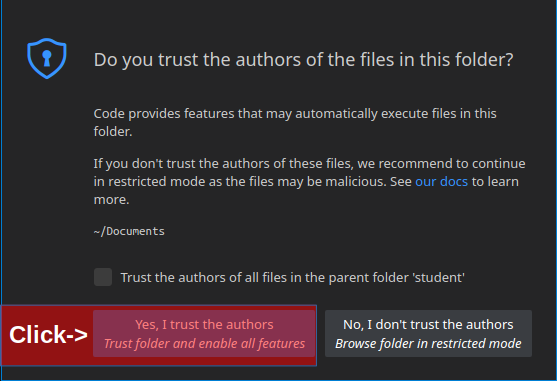
\includegraphics[width=0.5\textwidth]{pic_13}
\end{center}

\subsection{}Добавим путей для разрешения части include директив. Откройте .vscode -> c\_cpp\_properties.json
\begin{center}
	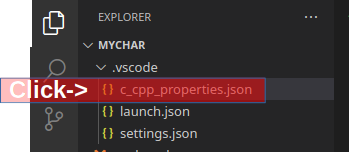
\includegraphics[width=0.5\textwidth]{pic_14}
\end{center}

\subsection{}Допишите в поле includePath следующие строки:\\
\begin{center}
	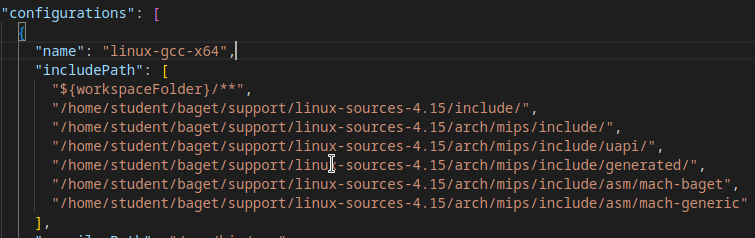
\includegraphics[width=\textwidth]{pic_15}
\end{center}
для удобства, воспользуйтесь файлом vscode\_lines.md в папке support. Ctrl+S для сохранения.

\subsection{}Изучите исходны код в файле spi\_temp.c. Для работы с SPI интерфейсом, в Linux есть готовые структуры, которые в данной работе используются. 

Из особенностей, которые хотелось бы отметить, это структура описание которой начинается с 11 строки. В ней описывается режим работы SPI интерфейса, в том числе номер интерфейса в системе. В нашем случае 1, так как 0 будет занят контроллером QSPI памяти.

Так же обратите внимание на организацию транзакции, описанную в функции  ext\_spi\_write (начало описания с 28 строки). В ней используется структура spi\_transfer, информацию о которой Вы можете получить, перейдя по ссылке 3 приведённой в начале лабораторной работы.

\subsection{}Перейдём в терминал (можно открыть вкладку TERMINAL в vscode, если её не видно, выберите в меню Terminal → New Terminal) и соберём модуль командой
\begin{lstlisting}[style=bash]
# ARCH=mips CROSS_COMPILE=mips64el-linux-gnuabi64- make 
\end{lstlisting}

\subsection{}Перейдём в терминал (можно открыть вкладку TERMINAL в vscode, если её не видно, выберите в меню Terminal → New Terminal) и соберём модуль командой
\begin{lstlisting}[style=bash]
	# ARCH=mips CROSS_COMPILE=mips64el-linux-gnuabi64- make 
\end{lstlisting}

\subsection{}Проверьте значение системной переменной BRD\_PASS  
\begin{lstlisting}[style=bash]
	# echo $BRD_PASS
\end{lstlisting}
если вывод был пустой, проинициализируйте переменную 
\begin{lstlisting}[style=bash]
	# export BRD_PASS="usrnetuser" 
\end{lstlisting}

\subsection{}Скопируйте модуль на плату
\begin{lstlisting}[style=bash]
	# ARCH=mips CROSS_COMPILE=mips64el-linux-gnuabi64- make install
\end{lstlisting}

\subsection{}Подключите модуль PmodALS как показано на рисунке 
\begin{center}
	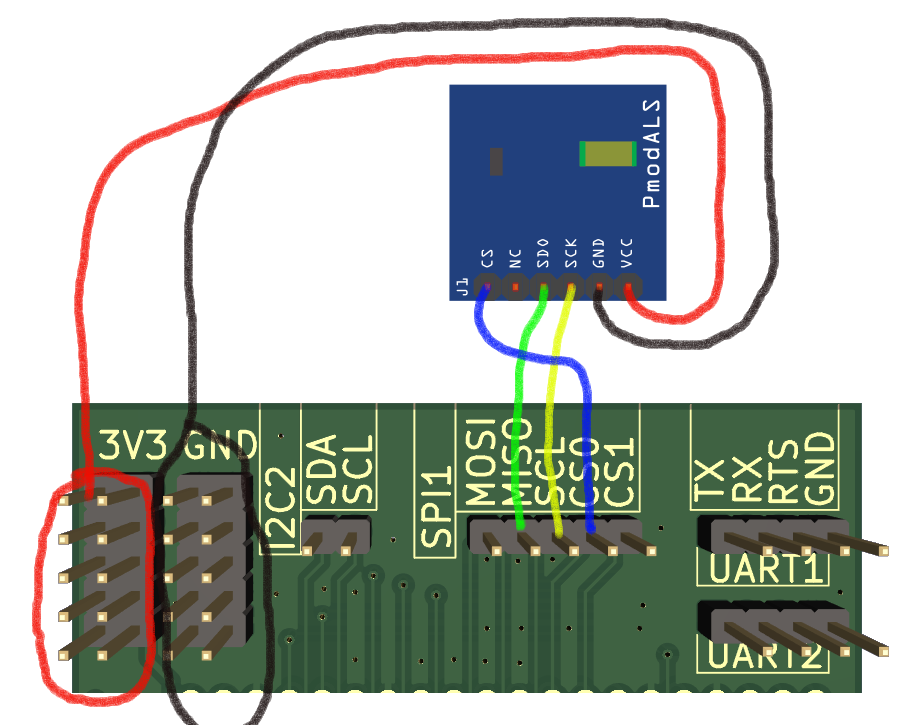
\includegraphics[width=0.7\textwidth]{pic_20}
\end{center}

\subsection{}Перейдите в терминал платы, и активируйте драйвера
\begin{lstlisting}[style=bash]
$ insmod /home/netuser/spi_temp.ko 
\end{lstlisting}

\subsection{}Вы должны увидите в терминале, информацию о том, что драйвер зарегистрирован, и 10 раз считано «сырое» значение освещённости с датчика.

\subsection{}Выгрузите драйвер командой
\begin{lstlisting}[style=bash]
$ rmmod spi_temp
\end{lstlisting}

\section{Задание для закрепления}
Внесите изменения в текущий драйвер таким образом, что бы создавался файл в папке /dev, чтение которого давало бы текущее значение освещённости.

В этом Вам может помочь код из лабораторной работы \ref{lab:char_dev}.

\subsubsection{*}
Внесите изменение в драйвер устройств таким образом, что бы частота, номер spi шины, и индекс вывода Chip Select передавались через описание в дереве устройств:
\begin{lstlisting}[style=stdout]
pmodals {
	compatible = "digilent,pmodals";
	spi_cfg = <400000 1 0>;	  
	status = "okay";
};
\end{lstlisting}
	%\include{lab_06}
	%\include{lab_07}
	%\include{lab_08}
	%\addcontentsline{toc}{chapter}{Список литературы}
\chapter*{Список литературы}

\begin{enumerate}
	\item Руководство для платы "<Багет-ПЛК1-01"> [Электронный ресурс] .- \\
	URL: \href{https://www.niisi.ru/%D0%91%D0%90%D0%93%D0%95%D0%A2-%D0%9F%D0%9B%D0%9A1-01_%D0%A0%D0%AD_v3.3.pdf}{https://www.niisi.ru/БАГЕТ-ПЛК1-01\_РЭ\_v3.3.pdf}
	
	\item Описание К5500ВК018 [Электронный ресурс] .- \\
	URL: \href{https://www.niisi.ru/%D0%9A%D0%BE%D0%BC%D0%B4%D0%B8%D0%B2-%D0%9C%D0%9A%20%D0%BE%D0%BF%D0%B8%D1%81%D0%B0%D0%BD%D0%B8%D0%B5%20v4.pdf}{https://www.niisi.ru/Комдив-MK\%20описание\%20v4.pdf}
	
	\item P. J. Salzman The Linux Kernel Module Programming Guide / Peter Jay Salzman, Michael Burian, Ori Pomerantz, Bob Mottram, Jim Huang [Электронный ресурс]. - URL: \href {https://sysprog21.github.io/lkmpg/}{https://sysprog21.github.io/lkmpg/}
	
	\item Навигатор по коду ядра Linux 4.15.18 [Электронный ресурс]. - \\
	URL: \href{https://elixir.bootlin.com/linux/v4.15.18/source}{https://elixir.bootlin.com/linux/v4.15.18/source}
	
	\item Документация ядра Linux 4.15 [Электронный ресурс]. - \\ 
	URL: \href{https://www.kernel.org/doc/html/v4.15/index.html}{https://www.kernel.org/doc/html/v4.15/index.html}
	
	\item  Спецификация Device Tree [Электронный ресурс]. - \\
	URL: \href{https://www.devicetree.org/specifications/}{https://www.devicetree.org/specifications/}
	
	\item Device Tree для «чайников» [Электронный ресурс]. - \\
	URL: \href{https://events.static.linuxfound.org/sites/events/files/slides/petazzoni-device-tree-dummies.pdf}{https://events.static.linuxfound.org/sites/events/files/slides/petazzoni-device-tree-dummies.pdf}
	
	\item  Руководство по установке Debian [Электронный ресурс]. - \\
	URL: \href{https://www.debian.org/releases/stable/armel/}{https://www.debian.org/releases/stable/armel/}
	
	\item  Спецификация разъёмов PMOD [Электронный ресурс]. - \\
	URL: \href{https://digilent.com/reference/\_media/reference/pmod/pmod-interface-specification-1\_2\_0.pdf}{https://digilent.com/reference/\_media/reference/pmod/pmod-interface-specification-1\_2\_0.pdf}
\end{enumerate}
\end{document}
